\hypertarget{mlp}{%
\subsubection{mlp}\label{mlp}}

Here is a conundrum. I'm using the \texttt{mlp} function to generate a
neural network to better fit the data. It's a beutiful fit actually, and
quite surprising for little data (perhaps becasue it has low noise?).
Still, I cannot seem to show that MSE \textbf{increases} as capacity
increases. It seems to be getting better\ldots{}

\begin{Shaded}
\begin{Highlighting}[]
\FunctionTok{set.seed}\NormalTok{(}\DecValTok{4723}\NormalTok{)}

\CommentTok{\#shuffle the data}
\NormalTok{df }\OtherTok{\textless{}{-}}\NormalTok{ earthquakes\_log[}\FunctionTok{sample}\NormalTok{(}\FunctionTok{nrow}\NormalTok{(earthquakes\_log)), ]}

\CommentTok{\#Extract 70\% of data into train set and the remaining 30\% in test set}
\NormalTok{train\_test\_split }\OtherTok{\textless{}{-}} \FloatTok{0.7} \SpecialCharTok{*} \FunctionTok{nrow}\NormalTok{(df)}
\NormalTok{train }\OtherTok{\textless{}{-}}\NormalTok{ df[}\DecValTok{1}\SpecialCharTok{:}\NormalTok{train\_test\_split,]}
\NormalTok{test }\OtherTok{\textless{}{-}}\NormalTok{ df[(train\_test\_split}\SpecialCharTok{+}\DecValTok{1}\NormalTok{)}\SpecialCharTok{:} \FunctionTok{nrow}\NormalTok{(df),]}

\NormalTok{mlp }\OtherTok{\textless{}{-}} \FunctionTok{neuralnet}\NormalTok{(freqc }\SpecialCharTok{\textasciitilde{}}\NormalTok{ mag,}
                 \AttributeTok{stepmax =} \FloatTok{1e+06}\NormalTok{,}
                 \AttributeTok{data =}\NormalTok{ train,}
                 \AttributeTok{hidden =} \FunctionTok{c}\NormalTok{(}\DecValTok{5}\NormalTok{,}\DecValTok{5}\NormalTok{))}

\CommentTok{\#prediction for magnitude 9.1}
\NormalTok{p }\OtherTok{\textless{}{-}} \FunctionTok{predict}\NormalTok{(mlp, }\AttributeTok{newdata =} \FunctionTok{data.frame}\NormalTok{(}\AttributeTok{mag =} \FloatTok{9.1}\NormalTok{))}
\DecValTok{1}\SpecialCharTok{/}\DecValTok{10}\SpecialCharTok{\^{}}\NormalTok{p}
\end{Highlighting}
\end{Shaded}

\begin{verbatim}
##          [,1]
## [1,] 3212.887
\end{verbatim}

\begin{Shaded}
\begin{Highlighting}[]
\CommentTok{\# \#predictions on test data}
\CommentTok{\# pps \textless{}{-} predict(mlp, newdata = data.frame(mag = test$mag))}
\CommentTok{\# }
\CommentTok{\# \#MSE to get test error}
\CommentTok{\# sum((pps {-} test$freqc)\^{}2)}


\CommentTok{\# {-}{-}{-} code to generate plot of predicted over actual data {-}{-}{-}}

\NormalTok{addt }\OtherTok{\textless{}{-}} \FunctionTok{seq}\NormalTok{(}\DecValTok{8}\NormalTok{,}\FloatTok{9.1}\NormalTok{, }\AttributeTok{by =}\NormalTok{ .}\DecValTok{1}\NormalTok{) }\CommentTok{\#additional magnitude data points to add to prediction data}

\CommentTok{\#{-}{-}{-}actual test data{-}{-}{-}}
\NormalTok{earthquakes\_p }\OtherTok{\textless{}{-}}\NormalTok{ earthquakes\_log[,}\FunctionTok{c}\NormalTok{(}\DecValTok{1}\NormalTok{,}\DecValTok{3}\NormalTok{)] }\SpecialCharTok{\%\textgreater{}\%} 
  \FunctionTok{mutate}\NormalTok{(}\AttributeTok{type =} \StringTok{"actual"}\NormalTok{) }\SpecialCharTok{\%\textgreater{}\%} 
  \FunctionTok{add\_row}\NormalTok{(}\AttributeTok{mag =}\NormalTok{ addt, }\AttributeTok{freqc =} \ConstantTok{NA}\NormalTok{, }\AttributeTok{type =} \StringTok{"actual"}\NormalTok{)}

\CommentTok{\#{-}{-}{-}predicted data{-}{-}{-}}
\NormalTok{magg }\OtherTok{\textless{}{-}}\NormalTok{ earthquakes\_log}\SpecialCharTok{$}\NormalTok{mag }\SpecialCharTok{\%\textgreater{}\%} \FunctionTok{append}\NormalTok{(addt) }\CommentTok{\#append additional magnitudes to make predictions}
\NormalTok{earthquakes\_p2 }\OtherTok{\textless{}{-}} \FunctionTok{data.frame}\NormalTok{(}\AttributeTok{mag =}\NormalTok{ magg,}
                             \AttributeTok{freqc =} \FunctionTok{predict}\NormalTok{(mlp, }\AttributeTok{newdata =} \FunctionTok{data.frame}\NormalTok{(}\AttributeTok{mag =}\NormalTok{ magg)),}
                             \AttributeTok{type =} \StringTok{"predicted"}\NormalTok{)}

\CommentTok{\#{-}{-}{-}combine test and predictions for plot{-}{-}{-}}
\NormalTok{plot }\OtherTok{\textless{}{-}} \FunctionTok{rbind}\NormalTok{(earthquakes\_p2,earthquakes\_p)}

\FunctionTok{ggplot}\NormalTok{(plot, }\FunctionTok{aes}\NormalTok{(}\AttributeTok{x =}\NormalTok{ mag, }\AttributeTok{y =}\NormalTok{ freqc, }\AttributeTok{group =}\NormalTok{ type, }\AttributeTok{color =}\NormalTok{ type)) }\SpecialCharTok{+}
  \FunctionTok{geom\_line}\NormalTok{() }\SpecialCharTok{+}
  \FunctionTok{geom\_point}\NormalTok{(}\AttributeTok{size =} \DecValTok{2}\NormalTok{, }\AttributeTok{shape =} \DecValTok{17}\NormalTok{ ) }\SpecialCharTok{+}
  \FunctionTok{theme\_minimal}\NormalTok{() }\SpecialCharTok{+}
  \FunctionTok{labs}\NormalTok{(}\AttributeTok{x =} \StringTok{"Magnitude"}\NormalTok{,}
       \AttributeTok{y =} \StringTok{"Annual Frequency of At Least this Magnitude"}\NormalTok{,}
       \AttributeTok{title =} \StringTok{"Annual Earthquake Frequency near Tohoku, Japan {-} Logarithmic Scale"}\NormalTok{,}
       \AttributeTok{subtitle =} \StringTok{"Three{-}Layer Neural Network"}\NormalTok{)}
\end{Highlighting}
\end{Shaded}

\begin{verbatim}
## Warning: Removed 12 rows containing missing values (`geom_line()`).
\end{verbatim}

\begin{verbatim}
## Warning: Removed 12 rows containing missing values (`geom_point()`).
\end{verbatim}

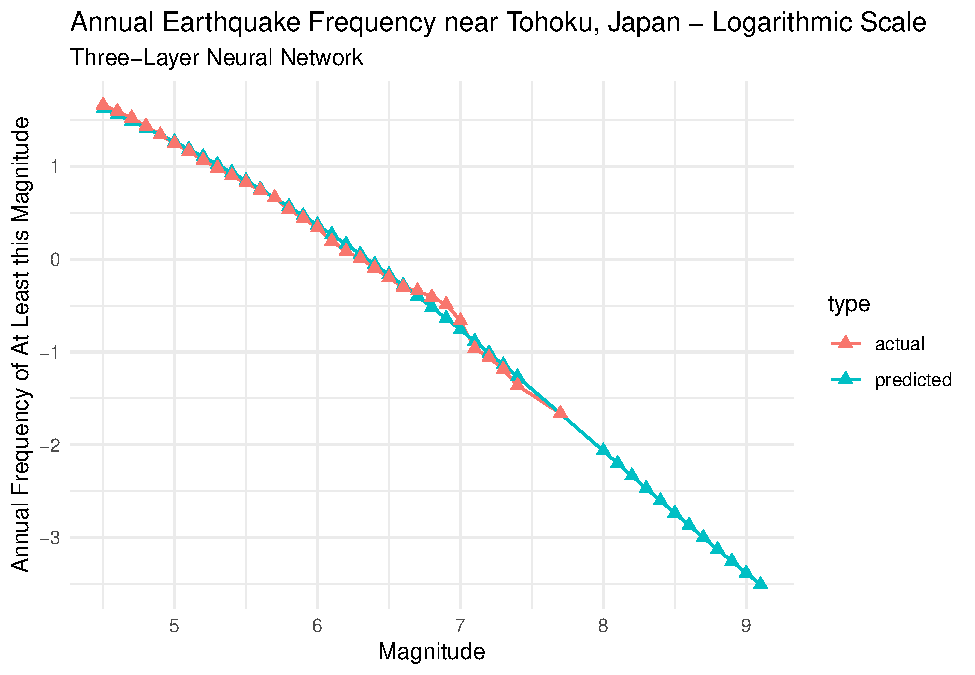
\includegraphics{earthquakes_files/figure-latex/unnamed-chunk-7-1.pdf}

\subsubbsection{testing capacity levels and MSE
measurements}

\begin{Shaded}
\begin{Highlighting}[]
\FunctionTok{set.seed}\NormalTok{(}\DecValTok{4723}\NormalTok{)}
\CommentTok{\#{-}{-}{-}one hidden layer{-}{-}{-}}
\NormalTok{mlp }\OtherTok{\textless{}{-}} \FunctionTok{neuralnet}\NormalTok{(freqc }\SpecialCharTok{\textasciitilde{}}\NormalTok{ mag,}
                 \AttributeTok{stepmax =} \FloatTok{1e+06}\NormalTok{,}
                 \AttributeTok{data =}\NormalTok{ train,}
                 \AttributeTok{hidden =} \FunctionTok{c}\NormalTok{(}\DecValTok{5}\NormalTok{))}

\CommentTok{\#predictions on test data}
\NormalTok{pps }\OtherTok{\textless{}{-}} \FunctionTok{predict}\NormalTok{(mlp, }\AttributeTok{newdata =} \FunctionTok{data.frame}\NormalTok{(}\AttributeTok{mag =}\NormalTok{ test}\SpecialCharTok{$}\NormalTok{mag))}

\CommentTok{\#SSE to get test error}
\NormalTok{SSE1 }\OtherTok{\textless{}{-}} \FunctionTok{sum}\NormalTok{((pps }\SpecialCharTok{{-}}\NormalTok{ test}\SpecialCharTok{$}\NormalTok{freqc)}\SpecialCharTok{\^{}}\DecValTok{2}\NormalTok{)}

\FunctionTok{set.seed}\NormalTok{(}\DecValTok{4723}\NormalTok{)}
\CommentTok{\#{-}{-}{-}two hidden layers{-}{-}{-}}
\NormalTok{mlp }\OtherTok{\textless{}{-}} \FunctionTok{neuralnet}\NormalTok{(freqc }\SpecialCharTok{\textasciitilde{}}\NormalTok{ mag,}
                 \AttributeTok{stepmax =} \FloatTok{1e+06}\NormalTok{,}
                 \AttributeTok{data =}\NormalTok{ train,}
                 \AttributeTok{hidden =} \FunctionTok{c}\NormalTok{(}\DecValTok{5}\NormalTok{,}\DecValTok{5}\NormalTok{))}

\CommentTok{\#predictions on test data}
\NormalTok{pps }\OtherTok{\textless{}{-}} \FunctionTok{predict}\NormalTok{(mlp, }\AttributeTok{newdata =} \FunctionTok{data.frame}\NormalTok{(}\AttributeTok{mag =}\NormalTok{ test}\SpecialCharTok{$}\NormalTok{mag))}

\CommentTok{\#SSE to get test error}
\NormalTok{SSE2 }\OtherTok{\textless{}{-}} \FunctionTok{sum}\NormalTok{((pps }\SpecialCharTok{{-}}\NormalTok{ test}\SpecialCharTok{$}\NormalTok{freqc)}\SpecialCharTok{\^{}}\DecValTok{2}\NormalTok{)}

\FunctionTok{set.seed}\NormalTok{(}\DecValTok{4723}\NormalTok{)}
\CommentTok{\#{-}{-}{-}three hidden layers{-}{-}{-}}
\NormalTok{mlp }\OtherTok{\textless{}{-}} \FunctionTok{neuralnet}\NormalTok{(freqc }\SpecialCharTok{\textasciitilde{}}\NormalTok{ mag,}
                 \AttributeTok{stepmax =} \FloatTok{1e+06}\NormalTok{,}
                 \AttributeTok{data =}\NormalTok{ train,}
                 \AttributeTok{hidden =} \FunctionTok{c}\NormalTok{(}\DecValTok{5}\NormalTok{,}\DecValTok{5}\NormalTok{,}\DecValTok{5}\NormalTok{))}

\CommentTok{\#predictions on test data}
\NormalTok{pps }\OtherTok{\textless{}{-}} \FunctionTok{predict}\NormalTok{(mlp, }\AttributeTok{newdata =} \FunctionTok{data.frame}\NormalTok{(}\AttributeTok{mag =}\NormalTok{ test}\SpecialCharTok{$}\NormalTok{mag))}

\CommentTok{\#MSE to get test error}
\NormalTok{SSE3 }\OtherTok{\textless{}{-}} \FunctionTok{sum}\NormalTok{((pps }\SpecialCharTok{{-}}\NormalTok{ test}\SpecialCharTok{$}\NormalTok{freqc)}\SpecialCharTok{\^{}}\DecValTok{2}\NormalTok{)}

\FunctionTok{data.frame}\NormalTok{(SSE1,SSE2,SSE3)}
\end{Highlighting}
\end{Shaded}

\begin{verbatim}
##          SSE1        SSE2       SSE3
## 1 0.009838334 0.008655795 0.01114061
\end{verbatim}

